\chapter{狄拉克海、费米子质量与四分量旋量}

\section{右行费米子与狄拉克海}

狄拉克方程是费米子所满足的方程。相对论性玻色子满足不同的方程，例如克莱因--戈尔登方程或麦克斯韦方程组。最简单的例子存在于一维空间中，最初描述的是只能向右运动的粒子与反粒子。

从平面波出发，
\begin{equation}
\psi(x,t)=\psi_0 e^{i(kx-\omega t)}.
\end{equation}
其相速度为
\begin{equation}
v_{\mathrm{ph}}=\frac{\omega}{k}.
\end{equation}
\(k\)与\(\omega\)的符号很重要。若二者同号，则相位向右移动；若二者异号，则相位向左移动。当\(\omega\)与\(k\)成正比时，相速度与群速度相等：
\begin{equation}
v_{\mathrm{g}}=\frac{d\omega}{dk}=\frac{\omega}{k}.
\end{equation}

考虑一阶方程
\begin{equation}
\frac{\partial\psi}{\partial x}
+
\frac{\partial\psi}{\partial t}
=0.
\end{equation}
代入平面波得到
\begin{equation}
ik\psi-i\omega\psi=0,
\end{equation}
因而
\begin{equation}
\omega=k.
\end{equation}
因此该波向右运动。相应地标记场是有用的：
\begin{equation}
\frac{\partial\psi_R}{\partial t}
=
-\frac{\partial\psi_R}{\partial x}.
\end{equation}

恢复光速后得到有量纲形式
\begin{equation}
\frac{\partial\psi_R}{\partial x}
+
\frac{1}{c}\frac{\partial\psi_R}{\partial t}
=0,
\end{equation}
于是
\begin{equation}
\omega=ck.
\end{equation}
从今以后取\(c=1\)。在\(\hbar=1\)下，\(\omega\)也是一个量子的能量。

\begin{figure}[htbp]
\centering
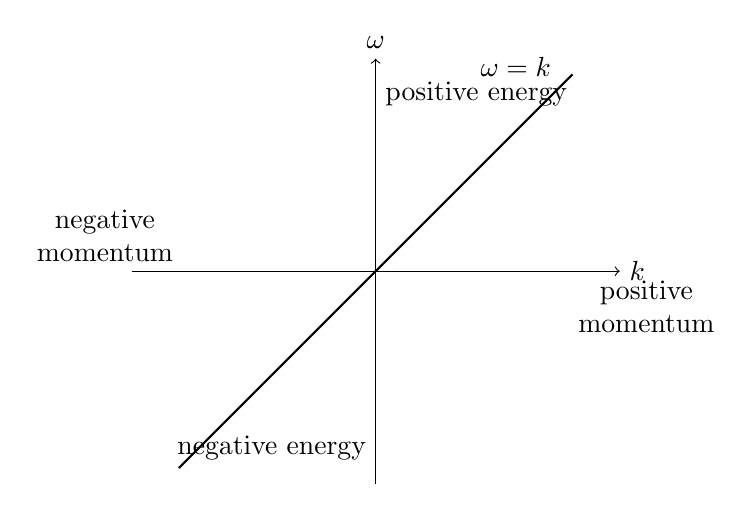
\begin{tikzpicture}[scale=1.0]
\draw[->] (-3.1,0) -- (3.1,0) node[right] {$k$};
\draw[->] (0,-2.7) -- (0,2.7) node[above] {$\omega$};
\draw[thick] (-2.5,-2.5) -- (2.5,2.5);
\node[above left] at (2.35,2.35) {$\omega=k$};
\node[below right,align=center] at (2.45,0) {positive\\momentum};
\node[above left,align=center] at (-2.45,0) {negative\\momentum};
\node[right] at (0,2.25) {positive energy};
\node[left] at (0,-2.25) {negative energy};
\end{tikzpicture}
\caption{无质量的右行色散关系\(\omega=k\)包含正能支与负能支。}
\end{figure}

这条直线有一个严重的后果。正的\(k\)给出正能，而负的\(k\)给出负能。然而两部分都描述向右运动的波，因为在整个直线上\(\omega/k=1\)。

置于正能部分的电子可以跃迁到较低的状态，发射一个正能光子，再次下落，并沿能谱继续下落：下一级台阶，再下一级，再下一级。没有电子会是稳定的。更严重的是，世界会通过产生越来越多的负能电子来降低自身能量。

费米子排斥原理提供了解决办法。填满每一个负能电子态。第二个电子不能进入已被占据的态，因此完全填满的负能区阻止了无限下落。这个被填满的区域就是狄拉克海，其完全填满的状态是基态，即真空。

\begin{classroomqa}
\lecturetimestamp{00:07:19}
\audiencequestion{是否存在无穷多个更低的负能态？}
\lecturerresponse{是的。对于离散动量，能谱像一架无限长的阶梯；对于连续动量，它像一条连续的滑梯。填满负能海阻止电子无限下落，不过当存在未被占据的更低状态时，仍可能发生伴随光子发射的有限向下跃迁。}
\end{classroomqa}

这解释了为什么具有这种能谱的方程必须被量子化为费米子理论。如果量子是玻色子，任意多个量子都可以占据同一个较低的状态，那么填满负能区并不能使真空稳定。

填满海的图像也产生反粒子。在真空中，所有负能级都被占据，所有正能级都空着。电子可以从任意一个被占据的负能级被激发到任意一个未被占据的正能级；初态和末态能级不必对称放置。

\begin{figure}[htbp]
\centering
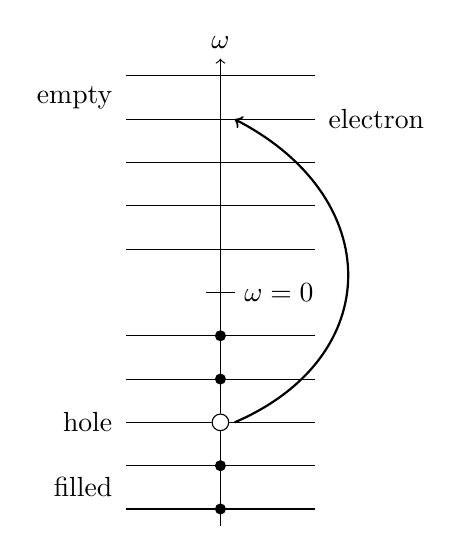
\begin{tikzpicture}[x=1cm,y=0.55cm]
\draw[->] (0,-5.4) -- (0,5.4) node[above] {$\omega$};
\draw (-0.18,0) -- (0.18,0) node[right] {$\omega=0$};
\foreach \y in {-5,-4,-3,-2,-1} {
  \draw (-1.2,\y) -- (1.2,\y);
  \fill (0,\y) circle (2pt);
}
\foreach \y in {1,2,3,4,5} {
  \draw (-1.2,\y) -- (1.2,\y);
}
\draw[->,thick] (0.18,-3) .. controls (2.1,-1.5) and (2.1,2.2) .. (0.18,4);
\draw[white,fill=white] (0,-3) circle (3pt);
\draw (0,-3) circle (3pt);
\node[left] at (-1.25,-3) {hole};
\node[left] at (-1.25,-4.5) {filled};
\node[left] at (-1.25,4.5) {empty};
\node[right] at (1.25,4) {electron};
\end{tikzpicture}
\caption{将一个被占据的负能电子激发出来，会产生一个正能电子，并在填满的海中留下一个空穴。}
\end{figure}

移走一个负能电子会使能量相对于真空升高，因此空穴具有正能。在\(\omega=k\)支上，被移走的电子也具有负动量。移走负动量会留下正的动量盈余，因此空穴具有正动量。取电子电荷为负，则缺失的电子具有正电荷。于是空穴是一个具有正能、正动量的反粒子，而被激发的电子具有负电荷、正能和正动量。在这个单支理论中，每一个真实的激发都向右运动。

场\(\psi_R\)由费米子产生与湮灭算符构成。因此，粒子与空穴的解释是关于场产生和移除的量子的一种陈述，而不仅仅是关于经典波的陈述。

仍然存在一种不对称性。右行海包含具有负动量的负能态。其形式上的总动量极其巨大，并且指向左方。人们可以通过减去这个常数来把真空动量定义为零，但该状态在结构上仍然不平衡：粒子与反粒子只向右运动，而被填满的真空却由负动量态构成。

\section{左行支与平衡的真空}

左右平衡要求存在第二个独立的场，它带有自己的产生和湮灭算符。令它满足
\begin{equation}
\frac{\partial\psi_L}{\partial t}
=
+\frac{\partial\psi_L}{\partial x}.
\end{equation}
对于相同的平面波形式，
\begin{equation}
-i\omega\psi_L=ik\psi_L,
\end{equation}
因此
\begin{equation}
\omega=-k.
\end{equation}
这第二行是\(\omega=k\)的镜像。其正能支描述向左运动的粒子，而其负能支也必须被填满。

\begin{figure}[htbp]
\centering
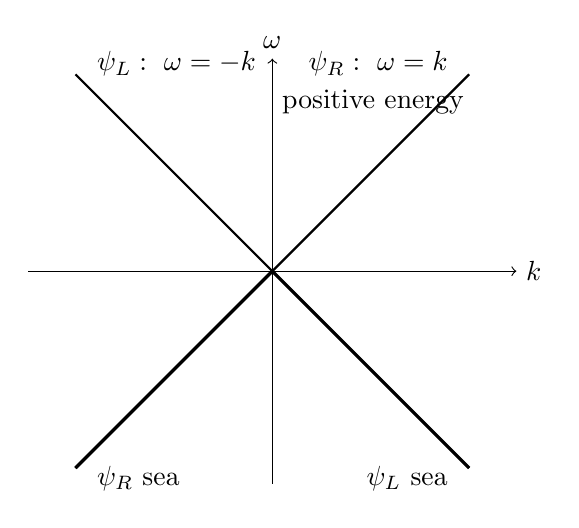
\begin{tikzpicture}[scale=1.0]
\draw[->] (-3.1,0) -- (3.1,0) node[right] {$k$};
\draw[->] (0,-2.7) -- (0,2.7) node[above] {$\omega$};
\draw[thick] (-2.5,-2.5) -- (2.5,2.5);
\draw[thick] (-2.5,2.5) -- (2.5,-2.5);
\draw[very thick] (-2.5,-2.5) -- (0,0);
\draw[very thick] (0,0) -- (2.5,-2.5);
\node[above left] at (2.35,2.35) {$\psi_R:\ \omega=k$};
\node[above right] at (-2.35,2.35) {$\psi_L:\ \omega=-k$};
\node[right] at (0,2.15) {positive energy};
\node[below right] at (-2.35,-2.35) {$\psi_R$ sea};
\node[below left] at (2.35,-2.35) {$\psi_L$ sea};
\end{tikzpicture}
\caption{独立的向右和向左运动的场给出互为镜像的无质量分支；两个负能半支在真空中被填满。}
\end{figure}

在填满两个负能海之后，向左运动和向右运动的占据态数目一样多。它们的真空动量相互平衡。粒子与空穴激发现在可以沿任一方向运动。

\begin{classroomqa}
\lecturetimestamp{00:15:58}
\audiencequestion{能否在不假设填满态和空穴的情况下处理负能问题？}
\lecturerresponse{同一理论可以重新标记。一个被填满的负能电子态可以称为一个空的反对粒子态；于是物理语言中只包含正能粒子和反粒子。填满海的图像仍然是一种有用的一致性检验，很像金属中的填满能带，其中移走一个电子产生一个空穴，而激发则同时产生一个粒子和一个空穴。}
\end{classroomqa}

到目前为止所考虑的激发都是无质量的。它们的色散关系是线性的，其速度大小为\(1\)，因此它们以光速运动。下一个问题是如何赋予它们质量。

\section{两个分量与质量项}

首先将两个场合并为一列：
\begin{equation}
\Psi=
\begin{pmatrix}
\psi_R\\
\psi_L
\end{pmatrix}.
\end{equation}
这最初只是两个独立方程的紧凑记号。定义
\begin{equation}
\alpha=
\begin{pmatrix}
1&0\\
0&-1
\end{pmatrix}.
\end{equation}
于是向右和向左运动的方程变为
\begin{equation}
\frac{\partial\Psi}{\partial t}
=
-\alpha\frac{\partial\Psi}{\partial x}.
\end{equation}

\begin{figure}[htbp]
\centering
\includegraphics[width=0.78\textwidth]{lecture_06_figure_02.png}
\caption{场\(\psi_R\)和\(\psi_L\)构成一个二分量旋量，其中\(\alpha\)区分两个无质量分支。}
\lectureframe{00:20:36}
\end{figure}

对于平面波，算符
\begin{equation}
i\partial_t
\quad\hbox{and}\quad
-i\partial_x
\end{equation}
分别返回\(\omega\)和\(k\)。因此矩阵方程可以简写为
\begin{equation}
\omega=\alpha k.
\end{equation}
对于上分量，这表示\(\omega=k\)；对于下分量，它表示\(\omega=-k\)。该记号压缩了两个方程，但没有引入任何新物理。

电子并非无质量，也不以光速运动。一个诱人的能量公式是非相对论动能\(k^2/(2m)\)，但这不能作为这里的出发点：无质量极限已经涉及以光速运动。相对论关系是
\begin{equation}
\omega^2=k^2+m^2,
\end{equation}
或者，包括两个能量分支，
\begin{equation}
\omega=\pm\sqrt{k^2+m^2}.
\end{equation}
当\(m=0\)时，它们约化为\(\omega=k\)和\(\omega=-k\)。

\begin{classroomqa}
\lecturetimestamp{00:25:23}
\audiencequestion{是否正在使用\(c=1\)的单位制，以及如何得到有质量粒子的速度？}
\lecturerresponse{是的。波包的速度是群速度，在正能支上为\(v_{\mathrm g}=d\omega/dk=k/\sqrt{k^2+m^2}\)。因此，色散关系本身已经包含了有质量粒子的速度降低到\(c=1\)以下。}
\end{classroomqa}

\begin{classroomqa}
\lecturetimestamp{00:26:29}
\audiencequestion{在简写\(\omega=\alpha k\)中，\(\omega\)是矢量还是矩阵？}
\lecturerresponse{该简写表示一个作用于二分量波函数的算符方程。这里\(\omega\)表示\(i\partial_t\)，\(k\)表示\(-i\partial_x\)，而\(\alpha\)是作用于分量指标的矩阵。标量符号\(\omega\)和\(k\)只有在平面波上才成为它们的数值本征值。}
\end{classroomqa}

保持方程为一阶，并尝试最简单的依赖于质量的扩展：
\begin{equation}
\omega=\alpha k+\beta m.
\end{equation}
对象\(\beta\)必须是矩阵，因为它与\(\alpha\)一样作用于同一个二分量场。其代数关系通过平方得到：
\begin{align}
\omega^2
&=(\alpha k+\beta m)(\alpha k+\beta m)\\
&=\alpha^2k^2+\beta^2m^2
+\alpha\beta\,km+\beta\alpha\,mk\\
&=\alpha^2k^2+\beta^2m^2
+(\alpha\beta+\beta\alpha)km.
\end{align}
为了对每个\(k\)和\(m\)都得到\(k^2+m^2\)，要求
\begin{equation}
\alpha^2=I,
\qquad
\beta^2=I,
\qquad
\alpha\beta+\beta\alpha=0.
\end{equation}

两个普通的非零数不可能满足最后一个条件：对于数，它会给出\(2\alpha\beta=0\)，与两个平方都为\(1\)相矛盾。矩阵可以反对易。特别地，\(\beta\)不能等于\(\alpha\)，因为那样
\begin{equation}
\alpha\beta+\beta\alpha=2\alpha^2=2I.
\end{equation}

选择
\begin{equation}
\beta=
\begin{pmatrix}
0&1\\
1&0
\end{pmatrix}.
\end{equation}
其平方可以逐项检验：
\begin{equation}
\begin{aligned}
\beta^2
&=
\begin{pmatrix}
0&1\\
1&0
\end{pmatrix}
\begin{pmatrix}
0&1\\
1&0
\end{pmatrix}\\
&=
\begin{pmatrix}
0\cdot0+1\cdot1&0\cdot1+1\cdot0\\
1\cdot0+0\cdot1&1\cdot1+0\cdot0
\end{pmatrix}
=
\begin{pmatrix}
1&0\\
0&1
\end{pmatrix}.
\end{aligned}
\end{equation}
乘法的顺序很重要：
\begin{align}
\alpha\beta
&=
\begin{pmatrix}
1&0\\
0&-1
\end{pmatrix}
\begin{pmatrix}
0&1\\
1&0
\end{pmatrix}
=
\begin{pmatrix}
0&1\\
-1&0
\end{pmatrix},\\
\beta\alpha
&=
\begin{pmatrix}
0&1\\
1&0
\end{pmatrix}
\begin{pmatrix}
1&0\\
0&-1
\end{pmatrix}
=
\begin{pmatrix}
0&-1\\
1&0
\end{pmatrix}.
\end{align}
因此
\begin{equation}
\alpha\beta=-\beta\alpha,
\qquad
\alpha\beta+\beta\alpha=0.
\end{equation}
其他等价的矩阵选择也是可能的，但这一选择使分量方程特别透明。

恢复微分算符后得到有质量方程
\begin{equation}
i\frac{\partial\Psi}{\partial t}
=
-i\alpha\frac{\partial\Psi}{\partial x}
+m\beta\Psi.
\end{equation}
矩阵\(\beta\)交换两个分量：
\begin{equation}
\beta
\begin{pmatrix}
\psi_R\\
\psi_L
\end{pmatrix}
=
\begin{pmatrix}
\psi_L\\
\psi_R
\end{pmatrix}.
\end{equation}
因此，
\begin{align}
i\dot{\psi}_R
&=-i\frac{\partial\psi_R}{\partial x}+m\psi_L,\\
i\dot{\psi}_L
&=+i\frac{\partial\psi_L}{\partial x}+m\psi_R.
\end{align}

质量项耦合了在无质量理论中原本相互独立的场。上分量的方程包含下分量，而下分量的方程包含上分量。这种耦合正是狄拉克质量的含义。这些方程具有平移不变性，因此它们守恒动量，而其粒子激发的质量为\(m\)。

\begin{classroomqa}
\lecturetimestamp{00:38:25}
\audiencequestion{一个解是否自动具有洛伦兹不变性？}
\lecturerresponse{一个特定的解不应在洛伦兹变换下保持不变。具有某一动量的态被变换为具有变换后动量的态，因此恰当的陈述是协变性。关系\(\omega^2=k^2+m^2\)是一个关键的洛伦兹不变性检验，但完整的协变性还要求旋量\(\Psi\)的变换律，而这一点尚未建立。}
\end{classroomqa}

\section{静止系与分量的含义}

无质量粒子不能被带到静止，但有质量粒子可以。在静止时\(k=0\)，因此波函数没有空间变化，并且
\begin{equation}
\omega=\beta m.
\end{equation}
微分方程简化为
\begin{equation}
i\frac{d\Psi}{dt}=m\beta\Psi.
\end{equation}
按分量写出，
\begin{align}
i\dot{\psi}_R&=m\psi_L,\\
i\dot{\psi}_L&=m\psi_R.
\end{align}
\(\beta\)的两个非对角元都是\(+1\)，因此这两个方程中都没有额外的负号。

将分量相加和相减后，方程解耦。定义
\begin{equation}
\psi_+=\psi_R+\psi_L,
\qquad
\psi_-=\psi_R-\psi_L.
\end{equation}
将两个静止系方程相加得到
\begin{equation}
i\dot{\psi}_+=m\psi_+,
\end{equation}
而将它们相减得到
\begin{equation}
i\dot{\psi}_-=-m\psi_-.
\end{equation}
因此
\begin{equation}
\omega=+m
\quad\hbox{for }\psi_+,
\qquad
\omega=-m
\quad\hbox{for }\psi_-.
\end{equation}

\begin{figure}[htbp]
\centering
\includegraphics[width=0.62\textwidth]{lecture_06_figure_03.png}
\caption{在零动量时，\(\psi_+=\psi_R+\psi_L\)和\(\psi_-=\psi_R-\psi_L\)具有静止频率\(\omega=+m\)和\(\omega=-m\)。}
\lectureframe{00:44:49}
\end{figure}

正能量的静止场是\(\psi_+\)；负能量的静止场是\(\psi_-\)。负能量态被填满，正如之前一样。静止系结果只是完整谱的\(k=0\)切片：
\begin{equation}
\omega_\pm(k)=\pm\sqrt{k^2+m^2}.
\end{equation}
\begin{figure}[htbp]
\centering
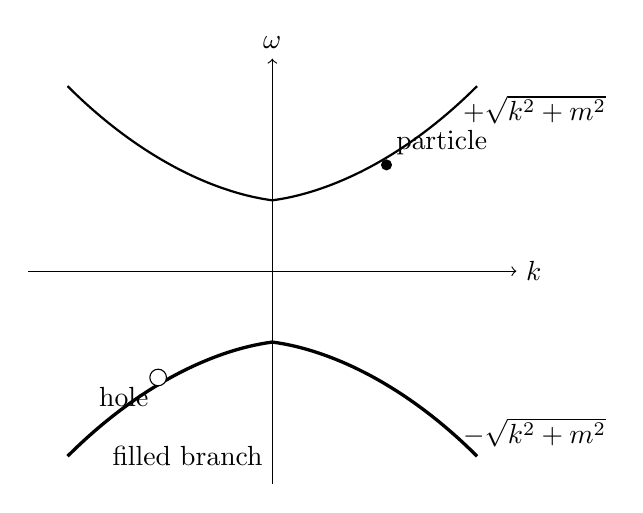
\begin{tikzpicture}[scale=1.0]
\draw[->] (-3.1,0) -- (3.1,0) node[right] {$k$};
\draw[->] (0,-2.7) -- (0,2.7) node[above] {$\omega$};
\draw[thick] (-2.6,2.35)
  .. controls (-1.7,1.45) and (-0.75,1.0) .. (0,0.9)
  .. controls (0.75,1.0) and (1.7,1.45) .. (2.6,2.35);
\draw[very thick] (-2.6,-2.35)
  .. controls (-1.7,-1.45) and (-0.75,-1.0) .. (0,-0.9)
  .. controls (0.75,-1.0) and (1.7,-1.45) .. (2.6,-2.35);
\fill (1.45,1.35) circle (2pt);
\node[above right] at (1.45,1.35) {particle};
\fill[white] (-1.45,-1.35) circle (3pt);
\draw (-1.45,-1.35) circle (3pt);
\node[below left] at (-1.45,-1.35) {hole};
\node[right] at (2.3,2.05) {$+\sqrt{k^2+m^2}$};
\node[right] at (2.3,-2.05) {$-\sqrt{k^2+m^2}$};
\node[left] at (0,-2.35) {filled branch};
\end{tikzpicture}
\caption{在每一个动量处，有质量谱都具有正能量态和负能量态。负能支被填满，其中缺失的态是正能量空穴。}
\end{figure}
每一个动量都有一个正能量态和一个负能量态。填满负能支上的每一个态，就在海之上留下正能量粒子，并在海中留下正能量空穴。粒子和空穴都具有正质量。

这一要点值得重复。当费米子的两个原本相互独立的分量被耦合时，它便获得质量。在静止时，单独任何一个原始分量都不是能量本征态。确定能量的态是它们的和与差。

为了看清这个和的含义，将相关的单粒子产生部分写作\(C_R^\dagger\)和\(C_L^\dagger\)。作用在真空上，
\begin{equation}
(C_R^\dagger+C_L^\dagger)\lvert0\rangle
\end{equation}
产生一个处于两个分量相干叠加中的粒子。它并不产生两个粒子。一个乘积，
\begin{equation}
C_R^\dagger C_L^\dagger\lvert0\rangle,
\end{equation}
包含两个产生算符，当两个模式都可用时产生一个两粒子态。归一化后，静止态在两个分量中具有相等的概率，但耦合后的波整体具有零动量。

标签\(R\)和\(L\)只有在\(m=0\)时才是字面意义上的运动标签。一旦存在质量项，运动的有质量解一般同时包含两个分量，而静止解以相等的幅度包含它们。因此，在这里最好将\(R\)和\(L\)视为旋量上分量和下分量的标签。

\begin{figure}[htbp]
\centering
\includegraphics[width=0.78\textwidth]{lecture_06_figure_04.png}
\caption{对于非零质量，两个旋量分量是耦合的；它们的右行和左行解释只在无质量极限下直接适用。}
\lectureframe{00:50:48}
\end{figure}

粒子物理学中所有有质量费米子都由左分量场和右分量场构成：狄拉克质量耦合了在无质量极限下相互独立的分量。

\begin{classroomqa}
\lecturetimestamp{00:52:01}
\audiencequestion{\(\psi_R\pm\psi_L\)是否应包含一个\(1/\sqrt{2}\)的因子？}
\lecturerresponse{可以包含它来归一化态。它乘在方程两边，因此不改变运动方程。}
\end{classroomqa}

\begin{classroomqa}
\lecturetimestamp{00:52:12}
\audiencequestion{右分量和左分量的相对大小重要吗？}
\lecturerresponse{对于所选的静止系本征态，它们的幅度相等。整体归一化是任意的，但相对幅度由\(\beta\)的本征矢固定。}
\end{classroomqa}

\begin{classroomqa}
\lecturetimestamp{00:52:52}
\audiencequestion{这两个分量之间可以有相对相位吗？}
\lecturerresponse{可以。\(\psi_R\pm\psi_L\)中的实系数来自选择实的\(\beta\)。其他平方等于单位矩阵且与\(\alpha\)反对易的矩阵是等价的选择，此时分量之间就可能出现相位。一旦选定了一种表示，就必须一致地使用它。}
\end{classroomqa}

\begin{classroomqa}
\lecturetimestamp{00:53:43}
\audiencequestion{在加入质量之后，``左行波''和``右行波''这些标签是否会误导？}
\lecturerresponse{有些会。它们描述的是无质量理论中真正的左行波和右行波。当质量非零时，即使一个沿某一方向运动的粒子通常也同时包含两个分量，因此``上分量''和``下分量''是更稳妥的标签。}
\end{classroomqa}

\begin{classroomqa}
\lecturetimestamp{00:55:01}
\audiencequestion{静止的费米子是否已经需要自旋角动量？}
\lecturerresponse{在这个一维模型中不需要。角动量在一维空间中未被定义，因此自旋尚未进入这一构造。}
\end{classroomqa}

\begin{classroomqa}
\lecturetimestamp{00:55:24}
\audiencequestion{波函数中是否包含费米子产生和湮灭算符？}
\lecturerresponse{是的。}
\end{classroomqa}

\begin{classroomqa}
\lecturetimestamp{00:55:30}
\audiencequestion{除了产生和湮灭算符的选择之外，费米子特性还从哪里进入？}
\lecturerresponse{它通过费米子产生--湮灭规则进入。具有这种负能谱的方程必须用这些规则量子化；玻色子占据规则会使真空不稳定。相对论性玻色子必须用不同的波动方程来描述。}
\end{classroomqa}

\begin{classroomqa}
\lecturetimestamp{00:56:20}
\audiencequestion{非零动量的解能否通过洛伦兹变换变成静止系的解？}
\lecturerresponse{可以。一个推动可以把有质量的解带到其静止系，但要实施这一变换，需要知道洛伦兹变换如何作用于旋量\(\Psi\)。}
\end{classroomqa}

\section{来自标量真空场的质量}

\begin{classroomqa}
\lecturetimestamp{00:58:11}
\audiencequestion{与希格斯场的相互作用如何产生狄拉克质量项？}
\lecturerresponse{把常数质量系数替换为与标量场的耦合。如果该场在真空中为零，费米子就仍然无质量；如果它具有恒定的非零真空值，该耦合的作用就完全像质量一样。}
\end{classroomqa}

设\(\phi(x,t)\)是一个具有自身运动方程的标量场。在狄拉克方程中，把质量项中的常数\(m\)替换为\(g\phi(x,t)\)：\footnote{所展示的相互作用项是通过在先前建立的质量项\(m\beta\Psi\)中作此替换而得到的。}
\begin{equation}
i\frac{\partial\Psi}{\partial t}
=
-i\alpha\frac{\partial\Psi}{\partial x}
+g\phi(x,t)\,\beta\Psi.
\end{equation}
于是这两个场方程耦合在一起。费米子作用于标量场，而标量场又反过来作用于费米子；合起来看，即使对于给定的\(\phi\)，狄拉克方程对\(\Psi\)是线性的，这个系统仍是非线性的。

首先假设空的空间具有
\begin{equation}
\phi(x,t)=0.
\end{equation}
那么混合项消失，上分量和下分量解耦，费米子无质量。反之，假设最低能量态具有恒定的非零标量场，
\begin{equation}
\phi(x,t)=\phi_0\neq0.
\end{equation}
该真空中的狄拉克方程变为
\begin{equation}
i\frac{\partial\Psi}{\partial t}
=
-i\alpha\frac{\partial\Psi}{\partial x}
+g\phi_0\,\beta\Psi,
\end{equation}
因此
\begin{equation}
m_{\mathrm{eff}}=g\phi_0.
\end{equation}
于是，玻色场与费米场之间的耦合，再加上空的空间中玻色场的非零值，产生了与先前直接写进方程中的质量相同的左右混合。

\begin{classroomqa}
\lecturetimestamp{01:01:27}
\audiencequestion{LHC能否为真空中的非零希格斯场提供证据？}
\lecturerresponse{绝对可以。那是重大问题之一。}
\end{classroomqa}

\begin{classroomqa}
\lecturetimestamp{01:01:32}
\audiencequestion{你能再多讲讲希格斯机制是如何起作用的吗？}
\lecturerresponse{标量场具有与其空间和时间变化相关的能量，它也可能具有局域势能\(V(\phi)\)。如果该势的极小值出现在\(\phi\)的非零值处，真空就包含非零场。围绕所选极小值的量子化振荡就是希格斯粒子。}
\end{classroomqa}

场可以以两种不同的方式携带能量。有些能量取决于场在空间和时间中如何变化。麦克斯韦场是熟悉的对照：
\begin{equation}
\mathcal{E}_{\mathrm{Maxwell}}\propto \mathbf E^2+\mathbf B^2,
\end{equation}
而\(\mathbf E\)和\(\mathbf B\)都由电磁势的导数构成。因此，这种能量与底层场的空间和时间变化相关。

标量场还可以具有局域势能密度，
\begin{equation}
V(\phi),
\end{equation}
它取决于 \(\phi\) 本身的值，而不是取决于它的导数。示意性地，
\begin{equation}
\mathcal{E}_\phi
=
\mathcal E_{\text{space and time gradients}}+V(\phi).
\end{equation}
如果没有更深的原理来确定它，\(V(\phi)\) 可以是任何与模型对称性相容的合理函数。

对于这里所使用的简化实标量示例，取该理论在
\begin{equation}
\phi\longrightarrow-\phi.
\end{equation}
下对称。于是势必须为偶函数：
\begin{equation}
V(\phi)=V(-\phi).
\end{equation}
仅凭这一对称性并不能说明最小值位于何处。一种可能是 \(\phi=0\) 处有一个单一最小值。另一种可能是在非零值处有一对对称的最小值，一个为正，一个为负。

\begin{figure}[htbp]
\centering
\includegraphics[width=0.72\textwidth]{lecture_06_figure_05.png}
\caption{位于 \(\phi=0\) 的最小值给出消失的真空场，而对称的非零最小值允许真空值 \(\phi_0\neq0\)，从而给出费米子质量 \(g\phi_0\)。}
\lectureframe{01:04:47}
\end{figure}

可以不指定势的具体多项式形式而画出这两种可能性。\footnote{下面的曲线只保留了论证中所用的定性上的居中最小值和对称相关最小值。}
\begin{figure}[htbp]
\centering
\resizebox{\linewidth}{!}{%
\begin{tikzpicture}[x=1.35cm,y=1.05cm]
\begin{scope}[shift={(-3.1,0)}]
\draw[->] (-1.7,0) -- (1.7,0) node[right] {$\phi$};
\draw[->] (0,-0.15) -- (0,2.45) node[above] {$V(\phi)$};
\draw[thick] (-1.5,2.05) .. controls (-0.9,0.65) and (-0.45,0.25) .. (0,0.25)
             .. controls (0.45,0.25) and (0.9,0.65) .. (1.5,2.05);
\fill (0,0.25) circle (1.2pt);
\node[below] at (0,0) {$0$};
\end{scope}
\begin{scope}[shift={(3.1,0)}]
\draw[->] (-1.7,0) -- (1.7,0) node[right] {$\phi$};
\draw[->] (0,-0.15) -- (0,2.45) node[above] {$V(\phi)$};
\draw[thick] (-1.55,2.05)
  .. controls (-1.25,0.75) and (-1.0,0.25) .. (-0.75,0.25)
  .. controls (-0.35,0.25) and (-0.25,1.3) .. (0,1.3)
  .. controls (0.25,1.3) and (0.35,0.25) .. (0.75,0.25)
  .. controls (1.0,0.25) and (1.25,0.75) .. (1.55,2.05);
\fill (-0.75,0.25) circle (1.2pt);
\fill (0.75,0.25) circle (1.2pt);
\node[below] at (0,0) {$0$};
\node[below] at (-0.75,0) {$-\phi_0$};
\node[below] at (0.75,0) {$\phi_0$};
\end{scope}
\end{tikzpicture}%
}
\caption{偶势可以具有居中的最小值，也可以具有两个对称相关的非零最小值。}
\end{figure}

如果最小值位于原点，则真空具有 \(\phi_0=0\)，而这种耦合不给电子质量。如果最小值位于 \(\phi=\pm\phi_0\)，则真空会落入其中任意一个。这两种选择由对称性相联系，并且二者都会在狄拉克方程中产生非零系数 \(g\phi_0\)。势为何具有这种定性形状是一个更深层的问题，并不能由该机制本身解决。

场不必恰好停留在其最小值处。它可以围绕所选值振荡，就像粒子可以在势阱底部附近振荡一样。将这些振荡量子化就得到希格斯量子。它们的特征频率与希格斯粒子质量有关：质量大意味着即使激发一个量子也需要大量能量。在真空中，场只是停留在其最小值附近并提供费米子质量。当场振动时，这种振动就是希格斯粒子。

这种耦合包含作用与反作用。费米子响应 \(\phi\) 的值，但能量足够高的费米子碰撞也可以激发标量场。碰撞必须提供激发能量；一旦场在振动，其量子就是希格斯粒子。同一个场不仅与电子耦合，也与夸克场以及其质量由它提供的其他场耦合。

\begin{classroomqa}
\lecturetimestamp{01:08:14}
\audiencequestion{如果希格斯场振动或发生位移，电子质量会改变吗？}
\lecturerresponse{会。由于有效质量与场的局域值成正比，使场向零位移会减小质量。将宏观区域保持在远离真空值处需要巨大能量；大到足以进行这种实验的区域可能会坍缩成黑洞。}
\end{classroomqa}

这个思想实验很直接。如果一个区域能够被保持在 \(\phi=0\) 附近，那么在该区域内
\begin{equation}
m_{\mathrm{eff}}=g\phi
\end{equation}
将变小或消失。受激的希格斯模式围绕真空值振荡，而在整个宏观区域内产生并维持可观的位移需要巨大能量。势能代价随体积增长。早在这样的区域成为实际实验室之前，其能量就可能大到足以发生引力坍缩。质量变化在原则上确实存在，但要安排一个大的可观测变化却极其困难。

\begin{classroomqa}
\lecturetimestamp{01:09:27}
\audiencequestion{为什么需要希格斯场？}
\lecturerresponse{因为电子有质量。}
\end{classroomqa}

\begin{classroomqa}
\lecturetimestamp{01:09:41}
\audiencequestion{每种粒子都有自己的希格斯场吗？}
\lecturerresponse{不。在标准模型中，一个希格斯场为电子、夸克以及参与这一机制的其他粒子提供质量。超对称版本需要两个希格斯场，而不是为每一种粒子各设一个独立的场。}
\end{classroomqa}

单场图像是示意性的：完整的希格斯场比单个实数 \(\phi\) 具有更多结构。尽管如此，要点仍然成立。一个共同的真空场可以以不同强度与不同费米子耦合，因此不同质量并不要求为每一种粒子各设一个不同的希格斯场。希格斯粒子就是同一个场围绕其真空值的振荡。

为什么不直接把电子质量手动放进方程中，而不要希格斯场呢？答案与弱相互作用和统一有关，此处暂不讨论。

\begin{classroomqa}
\lecturetimestamp{01:11:16}
\audiencequestion{在超对称理论中，是否存在两个希格斯部分？}
\lecturerresponse{是的。在此处使用的简化划分中，一个为 up 型夸克提供质量，另一个为 down 型夸克和电子提供质量。这种加倍是超对称性的技术要求，而不是每个粒子都有一个单独的希格斯场。}
\end{classroomqa}

\begin{classroomqa}
\lecturetimestamp{01:12:01}
\audiencequestion{如果希格斯粒子有质量，那么它的质量从何而来？}
\lecturerresponse{这个问题在此处并未解决。更尖锐的谜题是，为什么希格斯质量如此之小。}
\end{classroomqa}

对称性与质量问题密不可分。在简单的狄拉克模型中，一个阻止左、右部分混合的对称性会迫使混合项的系数为零。如果真空尊重该对称性，费米子将是无质量的。非零的希格斯真空值破坏了相关的真空对称性，并允许左右耦合：
\begin{equation}
m_{\mathrm{eff}}=g\phi_0\neq0.
\end{equation}
这里不展开精确的对称变换；要点在于它对质量项的后果。方程可能具有该对称性，尽管特定的最低能量态不具有。正是真空的这种不对称性提供了质量。

在正在勾勒的电弱图像中，电子和夸克以这种方式获得质量，\(W\) 和 \(Z\) 玻色子也是如此。光子保持无质量。希格斯粒子本身是另一个例外：即使没有相同的真空位移，它也可以有质量，而它的质量涉及自身场的振荡，而非左右费米子混合。因此，希格斯真空值在此叙述中生成了其他粒子的质量，而希格斯激发的质量则提出了一个单独的问题。

\begin{classroomqa}
\lecturetimestamp{01:15:26}
\audiencequestion{引力子有质量吗？}
\lecturerresponse{没有。引力子是无质量的，就像光子一样。中微子也曾被认为无质量，但它们具有非常小的质量；用当前的语言来说，这意味着它们的左、右分量之间只有非常小的耦合。}
\end{classroomqa}

光子和理论中的引力子都是无质量的，并以光速运动。中微子并不完全属于这一类。它们微小的质量意味着，在这种狄拉克语言中，连接其左、右分量的耦合非常微小。为什么它如此之小是另一个问题。

\section{三维空间中的狄拉克方程}

在三维空间中，波数变为波矢，
\begin{equation}
\mathbf{k}=(k_1,k_2,k_3),
\end{equation}
其分量沿 \(x\)、\(y\) 和 \(z\) 方向。一维关系具有符号
\begin{equation}
\omega=\alpha k+\beta m,
\end{equation}
其最简单的线性推广是
\begin{equation}
\omega
=
\alpha_1 k_1+\alpha_2 k_2+\alpha_3 k_3+\beta m.
\end{equation}
这里 \(\alpha_i\) 和 \(\beta\) 是矩阵。它们必须被选择为使
\begin{equation}
\omega^2=k_1^2+k_2^2+k_3^2+m^2.
\end{equation}
这个不变的色散关系是一个必要条件，尽管它本身并不是相对论的全部内容。

对线性表达式平方得到
\begin{align}
\omega^2
={}&
\alpha_1^2k_1^2+\alpha_2^2k_2^2+\alpha_3^2k_3^2+\beta^2m^2
\nonumber\\
&+(\alpha_1\alpha_2+\alpha_2\alpha_1)k_1k_2
+(\alpha_1\alpha_3+\alpha_3\alpha_1)k_1k_3
\nonumber\\
&+(\alpha_2\alpha_3+\alpha_3\alpha_2)k_2k_3
+\sum_{i=1}^{3}(\alpha_i\beta+\beta\alpha_i)k_i m.
\end{align}
平方动量与质量的系数要求
\begin{equation}
\alpha_1^2=\alpha_2^2=\alpha_3^2=I,
\qquad
\beta^2=I.
\end{equation}
不需要的 \(k_i k_j\) 项如果不同的 \(\alpha\) 矩阵反交换就会消失：
\begin{equation}
\alpha_i\alpha_j+\alpha_j\alpha_i=0,
\qquad i\neq j.
\end{equation}
混合的 \(k_i m\) 项如果
\begin{equation}
\alpha_i\beta+\beta\alpha_i=0
\qquad
\text{for each }i.
\end{equation}
就会消失。因此所有四个矩阵平方都等于单位矩阵，并且每一对不同的矩阵都反交换。

确实存在三个具有所需相互反交换性质的 \(2\times2\) 矩阵：它们就是三个泡利矩阵。不存在第四个既平方等于单位矩阵又与所有三个反交换的 \(2\times2\) 矩阵。\(3\times3\) 实现也不行。第一个可能的实现使用 \(4\times4\) 矩阵，即狄拉克矩阵。

从两个分量到四个分量的过渡提出了一个物理问题。在一维空间中，这两个分量最初是右行和左行场。四个分量意味着什么？新的要素将是自旋，但自旋需要角动量，因此需要一个真正的三维讨论。

这些矩阵不是唯一的。不同的选择是等价的，其方式与相互正交的坐标轴的不同选择是等价的非常相似：元素改变了，但一个变换联系着这些描述，物理不变。一个方便的表示是\footnote{下面逐元素的矩阵是紧接着展示的块形式与泡利矩阵的展开；那些块关系在讲座的 01:30:23--01:31:29 处被明确陈述。}
\begin{equation}
\beta=
\begin{pmatrix}
1&0&0&0\\
0&1&0&0\\
0&0&-1&0\\
0&0&0&-1
\end{pmatrix},
\end{equation}
连同
\begin{align}
\alpha_1&=
\begin{pmatrix}
0&0&0&1\\
0&0&1&0\\
0&1&0&0\\
1&0&0&0
\end{pmatrix},
&
\alpha_2&=
\begin{pmatrix}
0&0&0&-i\\
0&0&i&0\\
0&-i&0&0\\
i&0&0&0
\end{pmatrix},
\\[1ex]
\alpha_3&=
\begin{pmatrix}
0&0&1&0\\
0&0&0&-1\\
1&0&0&0\\
0&-1&0&0
\end{pmatrix}.
\end{align}
通过将每个矩阵分成 \(2\times2\) 块，它们的结构更容易看出：
\begin{equation}
\beta=
\begin{pmatrix}
I_2&0\\
0&-I_2
\end{pmatrix},
\qquad
\alpha_i=
\begin{pmatrix}
0&\sigma_i\\
\sigma_i&0
\end{pmatrix}.
\end{equation}
三个泡利矩阵是
\begin{equation}
\sigma_1=
\begin{pmatrix}
0&1\\
1&0
\end{pmatrix},
\quad
\sigma_2=
\begin{pmatrix}
0&-i\\
i&0
\end{pmatrix},
\quad
\sigma_3=
\begin{pmatrix}
1&0\\
0&-1
\end{pmatrix}.
\end{equation}
这些块矩阵满足所需的狄拉克反交换关系。

波函数现在必须有四个分量：
\begin{equation}
\Psi=
\begin{pmatrix}
\psi_1\\
\psi_2\\
\psi_3\\
\psi_4
\end{pmatrix}.
\end{equation}
运动方程为
\begin{equation}
i\frac{\partial\Psi}{\partial t}
=
-i\sum_{j=1}^{3}\alpha_j
\frac{\partial\Psi}{\partial x_j}
+\beta m\Psi.
\end{equation}
这个紧凑的表达式代表四个耦合的线性微分方程。\(\alpha_j\)的非对角元以比一维情形更复杂的方式混合这四个分量，但基本结构相同：矩阵耦合各分量，而方程在空间和时间上仍保持一阶。分量的额外加倍是导向自旋的线索。

\begin{classroomqa}
\lecturetimestamp{01:33:53}
\audiencequestion{\(\Psi\)的四个分量是直接与时空四个维度相关联的四维矢量吗？}
\lecturerresponse{不是。它们构成旋量，而不是四维矢量。在一维例子中，两个时空维度与两个旋量分量之间的相等是偶然的。在更高维的构造中，旋量矩阵的大小以二的幂次出现，一般不等于时空维数。}
\end{classroomqa}

静止系再次给出最简单的解释。在零动量时，导数项消失：
\begin{equation}
i\frac{\partial\Psi}{\partial t}=m\beta\Psi.
\end{equation}
在所选的表示中，\(\beta\)有两个本征值\(+1\)和两个本征值\(-1\)。因此有两个能量为\(+m\)的静止态和两个能量为\(-m\)的静止态。和之前一样，负能态被填满。每个能量符号内的二重多重性是额外结构，其物理解释就是自旋。

\begin{classroomqa}
\lecturetimestamp{01:35:51}
\audiencequestion{\(\alpha_i\)中的非对角块是否应带有相同的指标，使它们成为\(\sigma_i\)？}
\lecturerresponse{是的。每个矩阵\(\alpha_i\)在两个非对角块中都包含相应的泡利矩阵\(\sigma_i\)。}
\end{classroomqa}

\begin{classroomqa}
\lecturetimestamp{01:36:03}
\audiencequestion{\(\alpha_i\)的紧凑反对易关系中是否缺少一个因子二？}
\lecturerresponse{是的。当\(i=j\)时，左边是\(\alpha_i^2+\alpha_i^2=2I\)。正确的关系是\(\alpha_i\alpha_j+\alpha_j\alpha_i=2\delta_{ij}I\)。}
\end{classroomqa}

因此，分开的平方条件和不等指标条件可以合并为
\begin{equation}
\alpha_i\alpha_j+\alpha_j\alpha_i=2\delta_{ij}I.
\end{equation}

\begin{classroomqa}
\lecturetimestamp{01:36:42}
\audiencequestion{转向四个矩阵是狄拉克构造中的重大概念飞跃吗？}
\lecturerresponse{是的。狄拉克假设了该方程并追随其后果。一个后果是反粒子的出现；另一个是自旋。自旋在经验上早已为人所知，但该方程解释了它。}
\end{classroomqa}

\begin{classroomqa}
\lecturetimestamp{01:37:29}
\audiencequestion{是经验证据先出现，还是将粒子限制为玻色子和费米子的定理先出现？}
\lecturerresponse{经验证据先出现，定理后出现。玻色子--费米子二分法适用于三个空间维度。在两个空间维度和一个时间维度中，可以出现中间统计；在\(3+1\)维以及更高空间维度中，只有玻色子和费米子两种选择。}
\end{classroomqa}

\begin{classroomqa}
\lecturetimestamp{01:39:01}
\audiencequestion{\(\Psi\)的四个分量是否有惯用的指标？}
\lecturerresponse{这里没有固定本质性的选择。可以使用标记\(p\)和\(q\)，从一到四取值；这样每个矩阵就有一个行指标和一个列指标。}
\end{classroomqa}

矩阵记号隐藏了这些分量标记。如果将它们显露出来，则
\begin{equation}
p,q=1,2,3,4,
\end{equation}
方程读作
\begin{equation}
i\,\partial_t\Psi_p
=
-i\sum_{j=1}^{3}\sum_{q=1}^{4}
(\alpha_j)_{pq}\,\partial_j\Psi_q
+m\sum_{q=1}^{4}\beta_{pq}\Psi_q.
\end{equation}

\begin{classroomqa}
\lecturetimestamp{01:40:15}
\audiencequestion{当使用矩阵乘法时，显式的分量指标是不必要的吗？}
\lecturerresponse{是的。矩阵记号自动隐藏了那些指标。一个使相对论结构更显明的更对称形式可以在以后引入。}
\end{classroomqa}

所展示的方程是狄拉克方程最简单的\(3+1\)维形式。接下来的步骤是理解自旋，并构造相对论性玻色子的波动方程，因为狄拉克方程不是它们的方程，而自然界中大约一半的粒子是玻色子。有了这些要素，就可以转向夸克、轻子、弱玻色子、希格斯粒子和光子，并为粒子谱带来一些秩序。整个讨论中还需要更多对称性。